\section{Test \texorpdfstring{$\chi^2$}{chi quadro}}

Devi utilizzare questa sezione solo se il numero delle \textbf{osservazioni
      totale $n > 30$}.

\subsection{Dati senza Intervalli}

Devi utilizzare questa sezione solo quando hai dei dati \textbf{Senza
      Intervalli}, devi anche fare attenzione che il \textbf{numero di
      osservazioni $n > 30$}!!\\

Operazioni da effettuare:

\begin{enumerate}
      \item Riportare i dati in una tabella in Calc:
            \begin{itemize}
                  \item \textit{Colonna 1}: $categorie$
                  \item \textit{Colonna 2}: $f_i$
            \end{itemize}
      \item Raggruppare le categorie se $\exists \ categoria < 5$:
            \begin{itemize}
                  \item Parti dall'ultimo a salire (dal basso verso l'alto delle
                        categorie)
                  \item Raggruppale tutte nell'ultima categoria che le faccia
                        diventare maggiori di 5 sommando le frequenze.
                  \item \textit{Esempio}:
                        \begin{figure}[H]
                              \centering
                              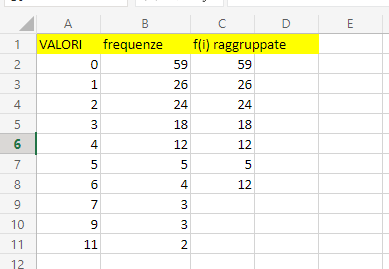
\includegraphics[width=6cm, keepaspectratio]{capitoli/goodnes_of_fit/imgs/vesceragay.png}
                              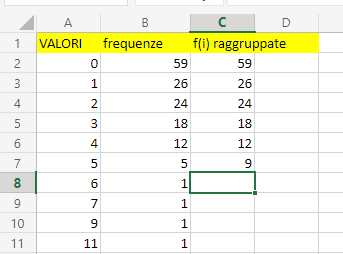
\includegraphics[width=5.5cm, keepaspectratio]{capitoli/goodnes_of_fit/imgs/POSTAMOLTOGAY.png}
                        \end{figure}
            \end{itemize}
      \item Calcolare:
            \begin{enumerate}
                  \item n = $\sum(f_i)$
                  \item \st{$f(i) = f_i / n$: non serve}
                  \item Capire la distribuzione se non è data (vedi
                        \ref{stimare-distribuzione})
                  \item $p(i)$: dipende dalla distribuzione (vedi \ref{pi})
                  \item $F_i = n * p(i)$: numero di intervalli unitari teorici
                        con $i$ arrivi
                  \item $G_i = \frac{(f_i - F_i)^2}{F_i}$
                  \item $V = \sum G_i$: sommare tutti i valori di $G$
                  \item $df = \text{Numero Categorie} - 1 - \text{Numero
                                    Parametri Distribuzione}$
            \end{enumerate}
\end{enumerate}

Una volta terminati i calcoli devi guardare la riga nella tabella del $\chi^2$
(AGGIUNGERE REF) con lo stesso valore di $df$: devi controllare che il valore
$V$ ricada negli intervalli che non superino il $P_{95}$.

\subsection{Dati con Intervalli}

Devi utilizzare questa sezione solo quando hai dei dati divisi in
\textbf{Intervalli}, devi anche fare attenzione che il \textbf{numero di
      osservazioni $n > 30$}!!\\

Calcoli da effettuare:

\begin{enumerate}
      \item Riportare i dati in una tabella in Calc:
            \begin{itemize}
                  \item \textit{Colonna 1}: $categorie$, probabilmente devi
                        aggiungerle tu, parti da 0 in poi
                  \item \textit{Colonna 2}: $intervallo$, del tipo $x_1 - x_2$.
                        Fai sempre attenzione che $x_2 \ge x_1$ !!! In caso li
                        inverti.
                  \item  \textit{Colonna 3}: $frequenza$ $f_i$
            \end{itemize}
      \item Aggiungere \textit{Colonna $x_1$} (intervallo più piccolo)
      \item Aggiungere \textit{Colonna $x_2$} (intervallo più grande)
      \item Aggiungere \textit{Colonna media-intervalli} tra \textit{$x_2$} e
            \textit{$x_1$}
      \item Calcolare:
            \begin{enumerate}
                  \item frequenze pesate = $\text{media-intervallo}_i * f_i$
                  \item $n$ = $\sum(f_i)$
                  \item media = $\sum(\text{frequenza pesata}_i)/n$
                  \item differenza medie = $(\text{media-intervalli}_i -
                              \text{media})^2$
                  \item frequenze pesate 2 = $\text{differenza media}_i * f_i$
                  \item frequenze relative = $f_i * n$
                  \item varianza $\sigma^2 = \sum(\text{frequenza pesata 2}_i) /
                              n - 1$
                  \item capire la distribuzione se non è data (vedi
                        \ref{stimare-distribuzione})
                  \item \st{$f(i) = f_i / n$: non serve}
                  \item $p(i) = p(x_2) - p(x_1)$ = calcolare secondo la distribuzione (vedi \ref{pi})
                  \item $F_i = n * p(i)$: numero di intervalli unitari teorici
                        con $i$ arrivi
                  \item $G_i = \frac{(f_i - F_i)^2}{F_i}$
                  \item $V = \sum G_i$: sommare tutti i valori di $G$
                  \item $df = \text{Numero Categorie} - 1 - \text{Numero
                                    Parametri Distribuzione}$
            \end{enumerate}
            %TODO: agli intervalli succede qualcosa ??
      \item Raggruppare le categorie se $\exists \ categoria < 5$:
            \begin{itemize}
                  \item Parti dall'ultimo a salire (dal basso verso l'alto delle
                        categorie)
                  \item Raggruppale tutte nell'ultima categoria che le faccia
                        diventare maggiori di 5 sommando le frequenze.
                  \item \textit{Esempio}:
                        \begin{figure}[H]
                              \centering
                              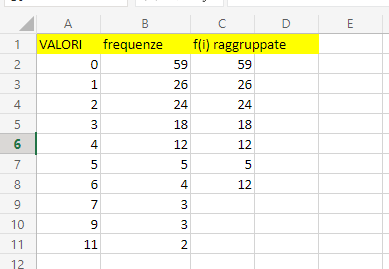
\includegraphics[width=6cm, keepaspectratio]{capitoli/goodnes_of_fit/imgs/vesceragay.png}
                              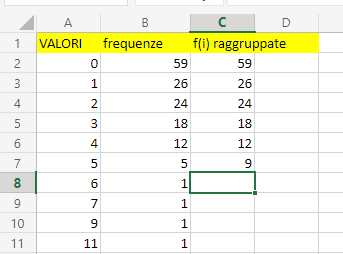
\includegraphics[width=5.5cm, keepaspectratio]{capitoli/goodnes_of_fit/imgs/POSTAMOLTOGAY.png}
                        \end{figure}
            \end{itemize}
\end{enumerate}

Una volta terminati i calcoli devi guardare la riga nella tabella del $\chi^2$
(AGGIUNGERE REF) con lo stesso valore di $df$: devi controllare che il valore
$V$ ricada negli intervalli che non superino il $P_{95}$.